\section{Аналитическая часть}

В данном разделе приводится краткий обзор предметной области. Описаны протоколы поддерживающие шифрование данных.


\subsection{Обзор предметной области}

\subsubsection{Модель OSI}

Модель OSI (Open Systems Interconnection) является концептуальным рамочным протоколом, разработанным Международной организацией по стандартизации (ISO), чтобы стандартизировать связь между различными компьютерными системами \cite{osi}. Она была определена в 1984 году и является основным принципом организации и реализации сетевых протоколов.

Модель OSI состоит из семи уровней, каждый из которых выполняет определенные функции для обеспечения надежной и эффективной коммуникации (см. рис \ref{fig:osi}).

\begin{figure}[h]
	\centering
	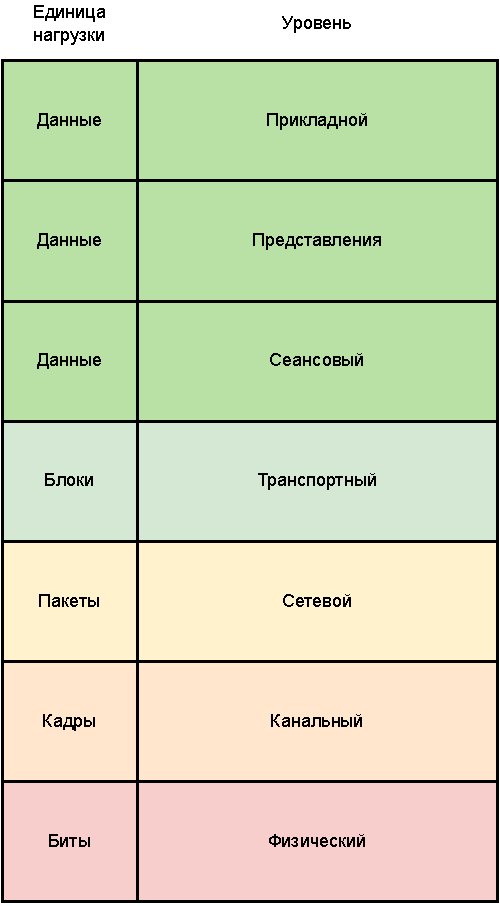
\includegraphics[scale=0.95]{img/osi.pdf}
	\caption{Модель OSI}
	\label{fig:osi}
\end{figure}

\begin{itemize}
	\item физический уровень: обеспечивает физическое соединение между устройствами и передачу битов по сети;
	\item канальный уровень: управляет надежной доставкой данных внутри локальной сети;
	\item сетевой уровень: обеспечивает маршрутизацию и передачу данных между различными сетями;
	\item транспортный уровень: отвечает за установление, управление и контроль надежной передачи данных между приложениями;
	\item сеансовый уровень: управляет установлением, поддержкой и завершением сеансов связи между устройствами;
	\item уровень представлений: обеспечивает преобразование данных в формат, понятный для приложений;
	\item прикладной уровень: предоставляет интерфейс для взаимодействия с приложениями.
\end{itemize}

Модель OSI широко используется при разработке и реализации сетевых протоколов, таких как Ethernet и многих других. Она обеспечивает стандартизацию и согласованность в связи между различными системами и является основополагающей моделью для понимания работы сетевых сред.

\subsubsection{Транспортный уровень}

Протокол, разработанный в рамках данной курсовой работы, находится на транспортном уровне модели OSI, поэтому далее будет дано его более подробное описание. 

Транспортный уровень является четвертым уровнем в сетевой архитектуре OSI. Он отвечает за передачу данных между конечными устройствами или хостами в сети. Основной задачей транспортного уровня является обеспечение эффективной и надежной передачи данных. Транспортный уровень представляет из себя функциональную надстройку над сетевым уровнем и решает две основных задачи:

\begin{enumerate}
	\item обеспечение доставки данных между конкретными программами, функционирующими, в общем случае, на разных узлах сети;
	\item обеспечение гарантированной доставки массивов данных произвольного размера.
\end{enumerate}

\subsubsection{Протоколы транспортного уровня}

Рассмотрим наиболее распространенные протоколы транспортного уровня: TCP (Transmission Control Protocol) \cite{TCP} и UDP (User Datagram Protocol) \cite{UDP}.

TCP является протоколом ориентированным на соединения. Он гарантирует доставку данных в правильном порядке и с контролем ошибок.

\begin{itemize}
	\item [---] TCP является соединительным протоколом. Он обеспечивает надежную, ориентированную на поток передачу данных между узлами в сети.
	\item [---] Для установления соединения TCP использует трехстороннее рукопожатие (three-way handshake), включающее отправку и получение пакетов SYN (synchronize) и ACK (acknowledge).
	\item [---] TCP контролирует порядок пакетов и гарантирует доставку данных без потерь, дублирования или повреждений.
	\item [---] Обеспечивает контроль нагрузки и управление потоком данных, чтобы избежать перегрузки сети.
	\item [---] TCP имеет встроенный механизм повторной передачи и контроля ошибок, что гарантирует целостность получаемых данных.
\end{itemize}

Протокол UDP используется в приложениях, где небольшие задержки более предпочтительны, например, в потоковой передаче видео и аудио. Основные особенности данного протокола:

\begin{itemize}
	\item [---] UDP является безсоединительным протоколом.
	\item [---] Не обеспечивает надежную доставку данных, контроль порядка пакетов или ретрансляцию потерянных пакетов.
	\item [---] UDP обеспечивает минимальное накладные расходы и более быструю передачу данных за счет отсутствия механизмов, используемых в TCP.
	\item [---] Он является хорошим выбором для приложений, где небольшие задержки важны, например, в реальном времени видео или голосовой связи.
	\item [---] Протокол UDP также удобен для широковещательной и многоадресной передачи данных.
	\item [---] В UDP-пакете нет гарантии доставки, но он прост и эффективен в простых сценариях, где периодическое обновление информации является приемлемым, а небольшие потери данных не критичны.
\end{itemize}

\subsubsection{Шифрование данных}

Шифрование данных является важным аспектом безопасности при передаче информации. Оно используется для защиты данных от несанкционированного доступа и предотвращения их изменения или подделки.

Шифрование данных может быть симметричным или асимметричным. В симметричном шифровании используется один и тот же ключ для шифрования и расшифрования данных.

Примерами симметричных алгоритмов шифрования является:

\begin{itemize}
	\item AES -- Advanced Encryption Standard \cite{AES};
	\item DES -- Data Encryption Standard \cite{DES}.
\end{itemize}

В асимметричном шифровании используется пара ключей: публичный и приватный. Публичный ключ используется для шифрования данных, а приватный ключ -- для их расшифровки. Это обеспечивает большую безопасность, так как приватный ключ хранится в секрете. Ниже представлены примеры наиболее популярных алгоритмов асимметричного шифрования:

\begin{itemize}
	\item RSA -- Rivest-Shamir-Adleman \cite{RSA};
	\item ECC -- Elliptic Curve Cryptography \cite{RSA};
	\item Diffie-Hellman \cite{RSA}. 
\end{itemize}

\subsection{Протоколы транспортного уровня с поддержкой шифрования}

\subsubsection{Secure Sockets Layer (SSL)}

SSL - это криптографический протокол для защиты передачи данных в сети. Он широко применяется в веб-браузерах, электронной почте, мгновенных сообщениях и IP-телефонии.

Протокол SSL обеспечивает следующие функции \cite{ssl}:

\begin{itemize}
	\item [---] Безопасность: данные защищаются симметричным шифрованием от несанкционированного доступа.
	\item [---] Аутентификация: можно проверить личность участников соединения с использованием асимметричного шифрования.
	\item [---] Целостность данных: протокол позволяет проверить, что данные не были изменены или потеряны в процессе передачи.
\end{itemize}

SSL работает в две фазы: рукопожатие и передача данных. Во время рукопожатия клиент и сервер используют открытый ключ для установки секретного ключа, который будет использоваться для шифрования данных во время передачи.

Рукопожатие начинается с того, что клиент отправляет <<hello>> сообщение серверу, содержащее список поддерживаемых клиентом алгоритмов шифрования. Сервер отвечает аналогичным <<hello>> сообщением, выбирая наиболее подходящий алгоритм из списка. Затем сервер отправляет свой сертификат, который содержит публичный ключ сервера.

Сертификат - это набор данных, который подтверждает подлинность. Доверенный центр сертификации генерирует и проверяет сертификат, чтобы удостовериться в его подлинности. Чтобы получить сертификат, сервер отправляет свой публичный ключ в центр сертификации по безопасному каналу. Сертификат содержит идентификаторы сервера, публичный ключ и другую информацию. Центр сертификации создает отпечаток сертификата, который является контрольной суммой, и подписывает сертификат с использованием своего приватного ключа.

Для проверки сертификата сервера клиент использует публичный ключ центра сертификации для расшифровки подписи. Затем клиент самостоятельно вычисляет отпечаток сертификата сервера и сравнивает его с расшифрованным значением. Если они не совпадают, то сертификат подделан. У клиента должен быть доступ к публичным ключам доверенных центров сертификации. Многие браузеры имеют такие списки в своем коде. Когда сервер аутентифицирован, он использует открытый ключ для установки секретного ключа для шифрования данных.

Фаза рукопожатия заканчивается отправкой <<finished>> сообщений, когда обе стороны готовы использовать секретный ключ. Начинается фаза передачи данных, в которой каждая сторона разбивает сообщения на фрагменты и добавляет к ним коды аутентификации сообщений (MAC). MAC является зашифрованным отпечатком, основанным на содержимом сообщений. Он вычисляется вместе с секретным ключом во время рукопожатия. Каждая сторона объединяет данные фрагментов, коды аутентификации сообщений, заголовки и шифрует их с использованием секретного ключа, чтобы создать полный пакет SSL. При получении пакета каждая сторона расшифровывает его и сравнивает полученный код аутентификации сообщения с собственным. Если они не совпадают, то пакет был подделан. На рисунке \ref{fig:ssl} представлена концептуальная схема работы SSL.

\begin{figure}[H]
	\centering
	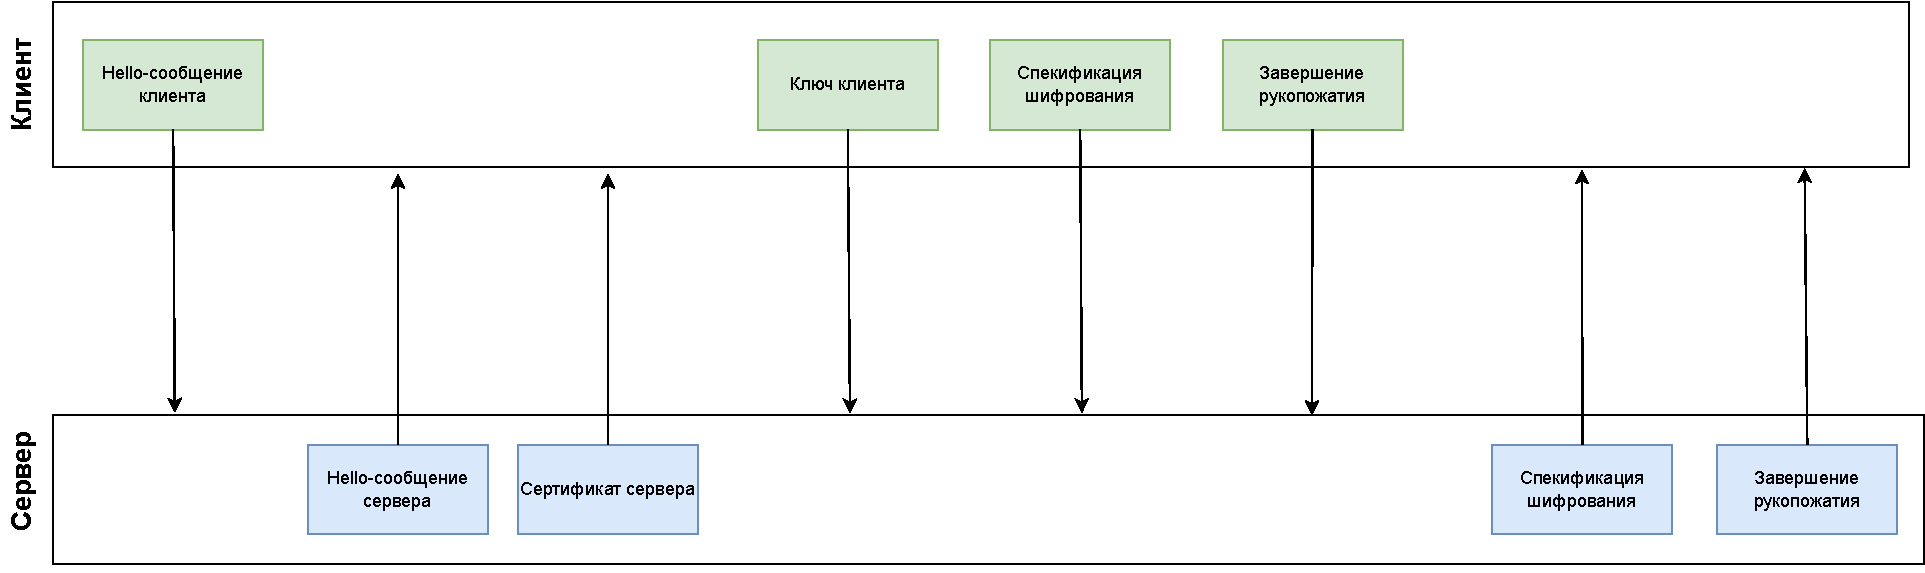
\includegraphics[scale=0.5]{img/ssl.pdf}
	\caption{Концептуальная схема работы SSL}
	\label{fig:ssl}
\end{figure}

SSL поддерживает 3 типа аутентификации:

\begin{enumerate}
	\item аутентификация обеих сторон (клиент — сервер);
	\item аутентификация сервера с неаутентифицированным клиентом;
	\item полная анонимность.
\end{enumerate}

Обычно для аутентификации используются алгоритмы: RSA и DSA. 

\subsubsection{Internet Protocol Security (IPSec)}

IPsec (Internet Protocol Security) - набор протоколов, которые взаимодействуют для обеспечения безопасной передачи IP-пакетов по незащищенным сетям.

IP-пакет - это блок данных, который передается по компьютерной сети и состоит из заголовка (с информацией об адресе отправителя и получателя и типе данных), полезной нагрузки (информация, передаваемая пользователем).

Протоколы IPsec обеспечивают \cite{ipsec}:

\begin{itemize}
	\item [---] Целостность данных -- защита от потери, изменения и дублирования при передаче.
	\item [---] Аутентичность отправителя -- гарантия, что данные были переданы от надежного источника;
	\item [---] Конфиденциальность — защита зашифрованных данных от несанкционированного просмотра.
\end{itemize}

Архитектурно IPsec состоит из 4 уровней \cite{ipsec}:

\begin{enumerate}
	\item аутентификация и шифрование данных;
	\item алгоритмы, использующиеся на первом уровне;
	\item домен интерпретации;
	\item создание политики безопасности соединения.
\end{enumerate}

На рисунке \ref{fig:ipsec} представлена архитектура IPsec.

\begin{figure}[h!]
	\centering
	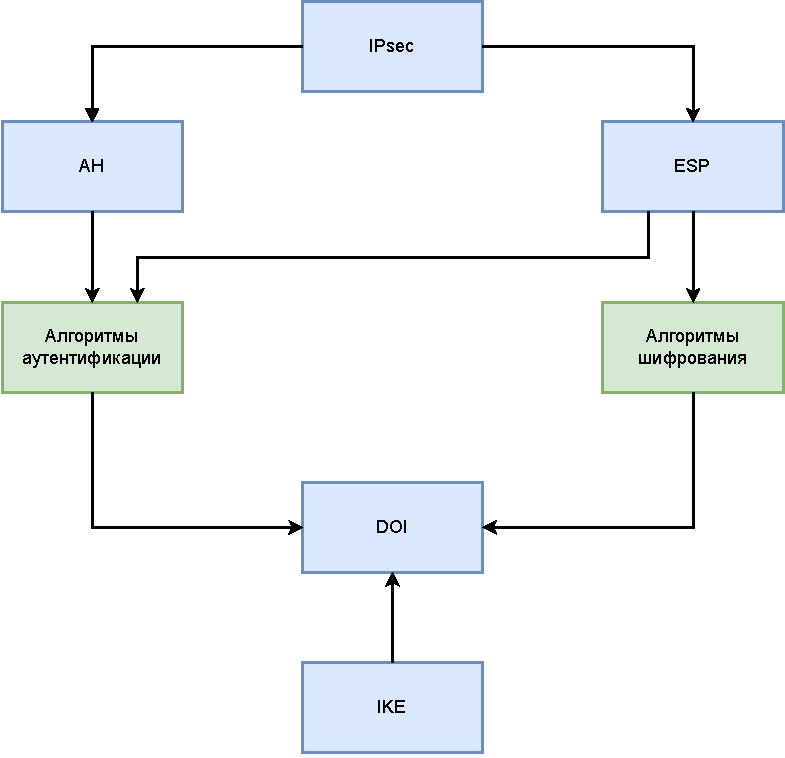
\includegraphics[width=\textwidth]{img/ipsec.pdf}
	\caption{Архитектура протокола IPSec}
	\label{fig:ipsec}
\end{figure}

На \textbf{первом уровне} находятся протоколы AH и ESP, которые гарантируют защиту данных на всех этапах их передачи. Они выполняют основные функции IPsec: аутентификацию, шифрование и являются ключевыми компонентами этой системы.

Протокол AH осуществляет:

\begin{enumerate}
	\item проверку подлинности: пользователь может удостовериться, что взаимодействует с ожидаемыми абонентами;
	\item целостность передаваемых данных: пользователь может обнаружить изменения данных в процессе передачи;
	\item защиту от повторного использования данных: данные не могут быть воспроизведены злоумышленниками.
\end{enumerate}

Протокол AH обеспечивает высокую степень защиты содержимого IP-пакета, поскольку предотвращает любые изменения в нем \cite{ah}. Однако это ограничивает его совместимость с сетевым режимом NAT (Network Address Translation), который изменяет IP-адреса при передаче IP-пакетов. Кроме того, в протоколе AH отсутствуют механизмы для защиты конфиденциальности передаваемых данных: злоумышленники не могут изменить данные, но могут их прочесть. Протокол ESP (Encapsulating Security Payload), подобно AH, поддерживает аутентификацию и целостность IP-пакета. Однако он также обеспечивает конфиденциальность передаваемых данных через шифрование. При этом применение всех этих функций для ESP не является обязательным, однако методы шифрования всегда необходимо использовать. Обычно протоколы ESP и AH используются независимо друг от друга, однако их комбинированное применение также возможно \cite{ah}.

Функции IPsec осуществляются конкретными алгоритмами, находящимися на \textbf{втором уровне} архитектуры. Аутентификация в IPsec реализуется при помощи специальных алгоритмов в протоколах AH и ESP. Например, для IPsec стандартные алгоритмы аутентификации HMAC используют общий секретный ключ для участников соединения \cite{hmac}. Алгоритмы HMAC обязательны для протокола AH и опциональны для ESP. Подробнее о процессе аутентификации можно прочитать в разделе Аутентификация в IPsec. Протокол ESP также поддерживает различные алгоритмы шифрования, включая DES, 3DES и AES. Это дополнительно усиливает защиту IP-пакета: для получения доступа к информации необходимо не только расшифровать данные, но и определить примененные алгоритмы шифрования. Подробнее о шифровании можно прочитать в разделе Шифрование в IPsec.

На \textbf{третьем уровне} находится DOI (домен интерпретации), который содержит информацию о примененных алгоритмах и протоколах. Использование DOI обусловлено тем, что протоколы AH и ESP могут поддерживать различные алгоритмы.

На \textbf{четвертом уровне} находится протокол IKE (Internet Key Exchange), который является основой IPsec. Он используется для установления политики безопасности соединения, таким образом отправитель и получатель согласовывают алгоритмы аутентификации и шифрования \cite{ike}. Кроме того, этот протокол обеспечивает генерацию и распределение ключей между участниками защищенного соединения.

\pagebreak
